\section{Organization and allocation of work}
\label{sec:organization}
\subsection{Two poles at about a thousand agents}
Microsoft Research's Agensh varies group size on software reconstruction tasks under a six-hour deadline \citep{agensh-1024}. Every team uses copies of GPT-5.6 Sol with the same prompt, its own Git branches, a shared chat, and an append-only context board on which an agent claims its part before starting. The logs describe negotiated interfaces at eight agents, reviewers chosen by experience and a shared merge protocol at 128, and self-appointed integrators at 1,024. On pandoc, the hidden-test score rises from 33.89\% for one worker to 55.06\% at 1,024; across five ProgramBench tasks, the mean rises from 19.31\% to 28.78\% between one and 128 agents. Token use is not compared. In the authors' published replay of the 1,024-worker run we count 11,111 successful pull-request creations, 2,800 merges, and 148,079 board writes, 56,472 of which carry the board label FAIL, a record type rather than a count of failed tasks; the replay's hash and our counting script are distributed with the report. The study shows that local agents can sustain differentiated coordination at this scale. With no matched designed hierarchy and no compute control, it establishes neither that emergence caused the gain nor that this organization was efficient.

Anthropic's Fable 5.2 run supplies the opposite pole at the same order of magnitude \citep{anthropic-fable-team-scaling}. The prompt set up one lead and 999 helpers, listed 60 statements to prove with 47 lemmas from the earlier formalization, and gave the agents no messaging tools; coordination passed through Git and a shared Postgres database. Within ten minutes the lead had created five tables for announcements, assignments, notes, subtasks, and finished work, and had assigned a crew of 16--17 helpers to each of 60 statements. After 27 minutes it set aside the 47 statements that most helpers had judged infeasible and regrouped crews of 46 to 139 helpers around the remaining ten. Authority did not stay central: by hour 5.6, 73 helpers had written 756 tasks, only 16 of them crew captains, and by the third hour the lead had told free helpers not to wait for assignments. For Langlands--Tunnell, a classical result that Wiles's proof relies on and by far the largest statement left in the run, the lead moved about 750 helpers onto one statement, and the task tree under it grew to 2,418 tasks up to ten levels deep. Agensh and the Fable run show emergent and designed authority with roughly a thousand agents, but on different tasks, models, and harnesses; the reviewed evidence contains no comparison of the two on a common task. Figure~\ref{fig:coordination} separates the layers such a comparison would need to hold apart: who can influence whom, through which medium, and how the organization arose.

The compiler campaign illustrates how emergent allocation depends on a designed substrate. Sixteen copies of a model reserve tasks through Git lock files and preserve notes across context resets. When all workers meet the same indivisible Linux-build failure, they duplicate fixes and interfere; a human-designed procedure that mixes the developing compiler with a reference compiler makes smaller independently testable subproblems available \citep{anthropic-c-compiler}. The Opus 5.5 developer evaluation adds a within-system contrast: a 100-agent Lean run develops two levels of communication with twelve retrospectively identified sub-leads, while a knowledge-base task remains relatively flat \citep{opus55-card}. Realized organization appears to respond to task dependencies, though neither study shows that the inferred structure was necessary.

\begin{figure*}[t]
\centering
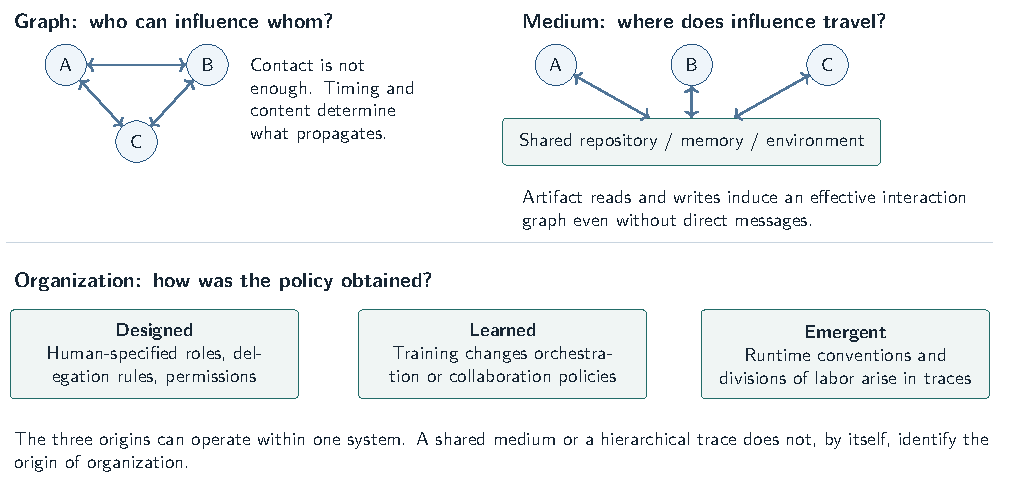
\includegraphics[width=\textwidth]{figures/coordination-layers.pdf}
\caption{Graph, medium, and organizational origin answer different questions about coordination. A shared repository can support either a designed hierarchy or an emergent allocation of work; the observed interaction graph must be measured separately. Original conceptual diagram by the report's human--AI collaboration.}
\label{fig:coordination}
\end{figure*}

\subsection{Allocation, integration, and authority}
Work allocation creates several distinct bottlenecks. Agents must discover an unclaimed task, judge whether it matters, avoid simultaneous ownership, and integrate the result. A system that solves task claiming may still fail at integration, and agents may make individually useful changes that conflict through an unstated design decision. CooperBench gives two agents overlapping coding features and compares them with one agent given both; chat reduces merge conflicts without recovering overall success \citep{cooperbench}. ParallACT (University of Texas at Austin and NVIDIA) builds pairs of requirements that contradict each other on purpose \citep{parallact-shared-codebases}. With Claude Code and Claude Opus 4.8, one agent that sees both requirements succeeds in 62\% of contradictory instances, while two agents that each see only their own reach 16\% under the best of three merge methods. Telling the pair that a peer works nearby raises joint success to 26\%, a difference that is not statistically significant.

Delivery of information is not the same as its use. In Worse Together, agents act for different users who share a resource \citep{worse-together,worse-together-blog}. In an API-token environment, peer teams reach 30\% (Claude Opus 5) and 12\% (Claude Sonnet 5) of the optimum, against 64\% and 32\% for a single coordinator. Across 25 personal-assistant scenarios, a user's request was sent to the agent that placed the final order in 94--99\% of episodes, yet it was in that agent's context at commit time in only 47--67\%. When it was in context, it was honored in 56--68\% of episodes; when it was not, in 19--36\%. The inbox study (MIT Media Lab) locates the bottleneck in reading rather than delivery \citep{inbox-coordination-primitive}. Its simulated societies reach 16,000 agents because agents shown the same information share one model answer, so a 16,000-agent run makes 6 to 23 model calls. In a separate experiment, an agent leading 20 negotiations with a full context proposes already rejected options 97\% of the time because it drops the oldest replies; under heavy, noisy traffic, an inbox with explicit reading rules becomes necessary.

Cursor's engineering history reports poor throughput from an early flat system and improved progress after recursive planning and isolated execution were introduced \citep{cursor-scaling-long-running,cursor-self-driving}. The comparison diagnoses locks, cautious local edits, and missing responsibility for cross-cutting changes; versions, prompts, models, and engineering experience changed together. Current products encode similar choices. Google Antigravity's /swarm passes a prompt to a coordinator that starts specialized workers in isolated Git worktrees together with adversarial verifiers \citep{google-antigravity-swarm}, and Google Research's Deep Review runs parallel review swarms over overlapping document segments before a global synthesis \citep{google-deep-review-october}. Neither post reports a controlled comparison with a single agent.

Authority solves some coordination problems and creates others. A manager's power to request revisions can add cost without improving the final report \citep{loop-back-authority}. Five Opus 5.5 peers reach intermediate ProgramBench targets sooner and with fewer tokens than the tested asynchronous hierarchy, with a similar final score \citep{opus55-card}, and DeLM's shared task queue and context can outperform its orchestrated comparator \citep{delm-shared-context}. The useful question is whether authority provides information, ownership, scheduling, or only another round of text generation; a role name does not say which.

\subsection{Learning rules before the task}
Self-Organizing Agent Teams revise their interaction strategy on training examples, then freeze a bank of strategies for evaluation \citep{sat-teams}. Their three-model reasoning team achieves 66.7\% across the reported mathematics and physics sets, against 48.8\% for its strongest ordinary individual and 58.7\% for an approximately budget-matched sequential execution of roles. On some held-out sets the latter margin narrows substantially, and on the knowledge-oriented suite it is nearly a tie. The predecessor study makes the mechanism plausible: role-free teams of strong and weak models fail to beat their strongest member, as nonexperts compromise and experts sometimes yield \citep{teams-hold-experts-back}.

Learning can also produce a local rule rather than an organization chart. Waggle (Shanghai Academy of AI for Science, Fudan University, and Yunnan University) learns one anonymous policy over bounded local views that selects actions, messages, and commitments for interchangeable agents \citep{waggle-2026}. According to the authors' summary, the learned law remains effective as populations and interaction budgets change, retains over 96\% of the quality of substrate-specific oracles, and transfers without retraining. Avalon-M1 shows how a trained organization changes its plans: over training on a collective reward, opening plans that split work by component fall from 71\% to 31\%, while build, test, and review pipelines around one code owner rise from 16\% to 54\% \citep{avalon-m1}. Learned controllers such as Conductor and TRINITY choose models or roles with policies optimized outside the evaluation \citep{sakana-conductor,sakana-trinity}, and search over heterogeneous role assignments belongs to the same design space \citep{heterogeneous-swarms}. Such training automates organizational design, yet the resulting runtime system can still be centralized: decentralization, adaptivity, and automation are separate properties.

Coordination without shared training remains weak. In minimal environments built to isolate specific coordination problems, independently developed frontier agents struggle to coordinate, largely because they misread the coordination problem and their partner's beliefs \citep{zero-shot-coordination-2026}.

\subsection{Organization as an experimentally testable object}
A useful organizational ablation holds the model pool and total budget fixed while changing one allocation mechanism: replacing task claims with a scheduler, enforcing a message-read barrier, separating planner and writer, or removing a reviewer. It should measure duplicate work, waiting time, stale dependencies, merge failures, and accepted improvements in addition to final success. New benchmarks make such ablations easier. MASBench varies collaboration mechanisms under partial observability \citep{masbench-2026}, and World of SWECraft simulates agents that maintain interdependent Python packages, where enabling collaboration helps some model families and has unclear effects for others \citep{world-of-swecraft}.

Human interventions must be logged at the same level. Choosing the initial decomposition, redirecting a search, introducing a verifier, and restarting agents are different contributions; the Fable run, for example, sent the lead 19 automatic reminders about the remaining time and was restarted from a save near hour 18 \citep{anthropic-fable-team-scaling}. Large demonstrations disclose some interventions but rarely a complete timeline. A fair report can credit the collective's achievements while leaving the advantage of its organizational form unresolved.
